%%==================================================
%% chapter04.tex for SJTU Master Thesis
%% based on CASthesis
%% modified by wei.jianwen@gmail.com
%% version: 0.3a
%% Encoding: UTF-8
%% last update: Dec 5th, 2010
%%==================================================

% \bibliographystyle{sjtu2} %[此处用于每章都生产参考文献]

\chapter{系统实现}
\label{chap:system}

\section{GSM-R网络空中接口测试}
\label{sec:um}

The algorithm design and implementation is presented in this section, which first gives a brief description of on-line measurement procedure and then demonstrates the software framework and development.

\begin{algorithm}[!htp]
%\floatname{algorithm}{Procedure}
\renewcommand{\algorithmicrequire}{\textbf{Input:}}
\renewcommand{\algorithmicensure}{\textbf{Output:}}
\caption{On-line estimation of local mean power in Rician fading channels}
\label{alg:online}
\begin{algorithmic}[1]
\Require $v_{train}$, $r_i$, $\nu_k$, $\sigma_k$
\Ensure  $\nu_{k+1}$, $\sigma_{k+1}$, $2L$, $N$, $\Delta d$
\State {// 1. The initialization of $\nu$ and $\sigma$.}
\If {begin-flag==true}
\State {$\Delta d$ $\leftarrow$ Lee($2L_0$,$N_0$;$\lambda$);}
\State {\{$\nu_{last}$, $\sigma_{last}$\} $\leftarrow$ EM($\Delta d$,$N_0$;$r_i$); // Equation(\ref{nu_0}),(\ref{sigma_0})}
\State {\{$\nu_{now}$, $\sigma_{now}$\} $\leftarrow$ EM($\Delta d$,$N_0$;$r_i$;$\nu_{last}$,$\sigma_{last}$); // Equation(\ref{EM_nu}),(\ref{EM_sigma})}
\While {($\nu_{now}-\nu_{last}>\nu_{thr}$) \& ($\sigma_{now}-\sigma_{last}>\sigma_{thr}$)}
\State {\{$\nu_{next}$, $\sigma_{next}$\} $\leftarrow$ EM($\Delta d$,$N_0$;$r_i$;$\nu_{now}$,$\sigma_{now}$); // Equation(\ref{EM_nu}),(\ref{EM_sigma})}
\State {$\{\nu_{last},\sigma_{last}\} \leftarrow \{\nu_{now},\sigma_{now}\}$;}
\State {$\{\nu_{now},\sigma_{now}\} \leftarrow \{\nu_{next},\sigma_{next}\}$;}
\EndWhile
\State {$2L_{now} \leftarrow f_{2L}(\lambda;,\nu_{now},\sigma_{now})$; // Equation(\ref{Perror})}
\State {$N_{now} \leftarrow f_{N}(\nu_{now})$; // Equation(\ref{Qerror})}
\EndIf
\State {// 2. On-line estimation of $\nu$ and $\sigma$, determination of $2L$, $N$ and $\Delta d$.}
\If {operating-flag==true}
\For {$i=0;i<N_{now};i++$}
\State {\{$\nu_{next}$, $\sigma_{next}$\} $\leftarrow$ EM($\Delta d$,$N_0$;$r_i$;$\nu_{now}$,$\sigma_{now}$); // Equation(\ref{EM_nu}),(\ref{EM_sigma})}
\State {$2L_{next} \leftarrow f_{2L}(\lambda;,\nu_{now},\sigma_{now})$; // Equation(\ref{Perror})}
\State {$N_{next} \leftarrow f_{N}(\nu_{now})$; // Equation(\ref{Qerror})}
\State {$\Delta d_{next} = f_{2L}(\lambda;,\nu_{now},\sigma_{now})/f_{N}(\nu_{now})$;}
\State {$\{\nu_{last},\sigma_{last};2L_{last},N_{last}\} \leftarrow \{\nu_{now},\sigma_{now};2L_{now},N_{now}\}$;}
\State {$\{\nu_{now},\sigma_{now};2L_{now},N_{now}\} \leftarrow \{\nu_{next},\sigma_{next};2L_{next},N_{next}\}$;}
\If {$i==N_{last}$}
\State {i=0;}
\EndIf
\EndFor
\EndIf
\end{algorithmic}
\end{algorithm}

The on-line estimation algorithm is given in Algorithm~\ref{alg:online}, which is based on the derivation and calculation introduced in the previous section. First, the initialization is conducted to calculate the initial value of Rician fading factors $\nu_0$ and $\sigma_0$. It is calculated by EM algorithm with the statistical interval length $2L=40\lambda$ and averaging sample numbers $N=36$. Then $\nu_k$ and $\sigma_k$ are estimated in every $k$-th compute cycle based on the estimation results of the last round. At the same time, the averaging factors $2L$ and $N$ of next cycle are calculated based on the measurement samples and Rician fading factors. Finally, the sampling interval is determined by $\Delta d=2L/N$, which can be converted to the time scale by the current velocity of train $v_{train}$. The process of received signal strength sampling and fading channels factors estimation is conducted in each compute cycle.

\begin{figure}[!htp]
%\onelinecaptionsfalse
\centering
    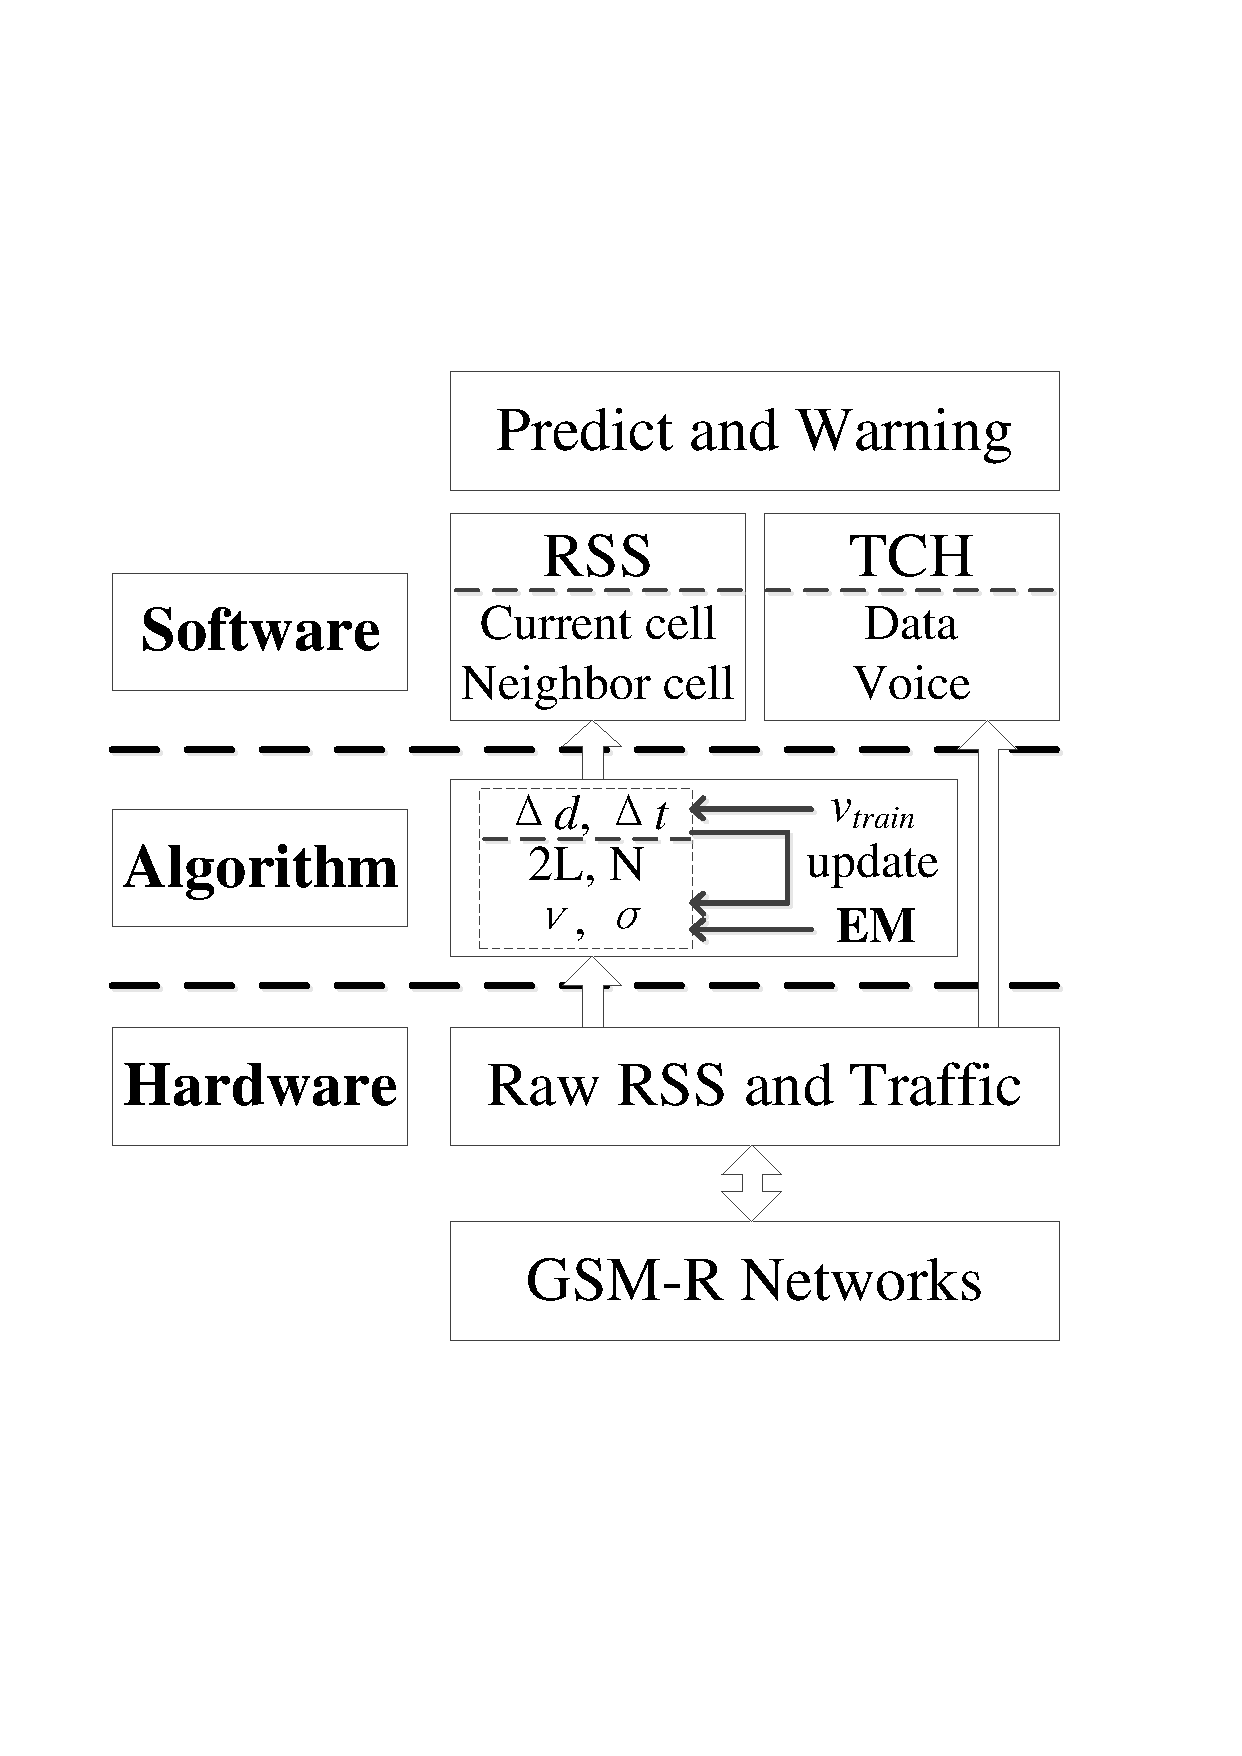
\includegraphics[width=4in]{chap5/umframework.pdf}
\bicaption[fig:umframework]{信道状态估计算法与实现}{信道状态估计算法与实现}{Fig}{Estimation framework and algorithm implementation}
\end{figure}

To get the received data and evaluate the measurement performance, we developed the Um interface monitoring system for GSM-R networks. The hardware and software architecture is shown in Fig.~\ref{fig:platform}, and the online estimation algorithm is implemented on this platform. The system's cpu module is RTD's CME137686LX-W including a 333MHz AMD Geode LX processor with 128kB L1 cache and 128kB L2 cache, and the communication module is COM16155RER-1 using Triorail's GSM-R engine TRM:3a. The system's power supply, processor and comunication module are connected through PC/104 bus, and other peripherals through its specific interface. The hardware components is demonstrated in Fig.~\ref{fig:hardware}. The software is independently developed by our research group, which uses Microsoft .NET Compact Framework in C\#, and it can run on various operating systems including Windows XP, Windows Mobile, and Windows CE. The software interface is shown in Fig.~\ref{fig:software}.

\begin{figure}[!htp]
\centering
\subfigure[Hardware Design]{
    \label{fig:hardware}
    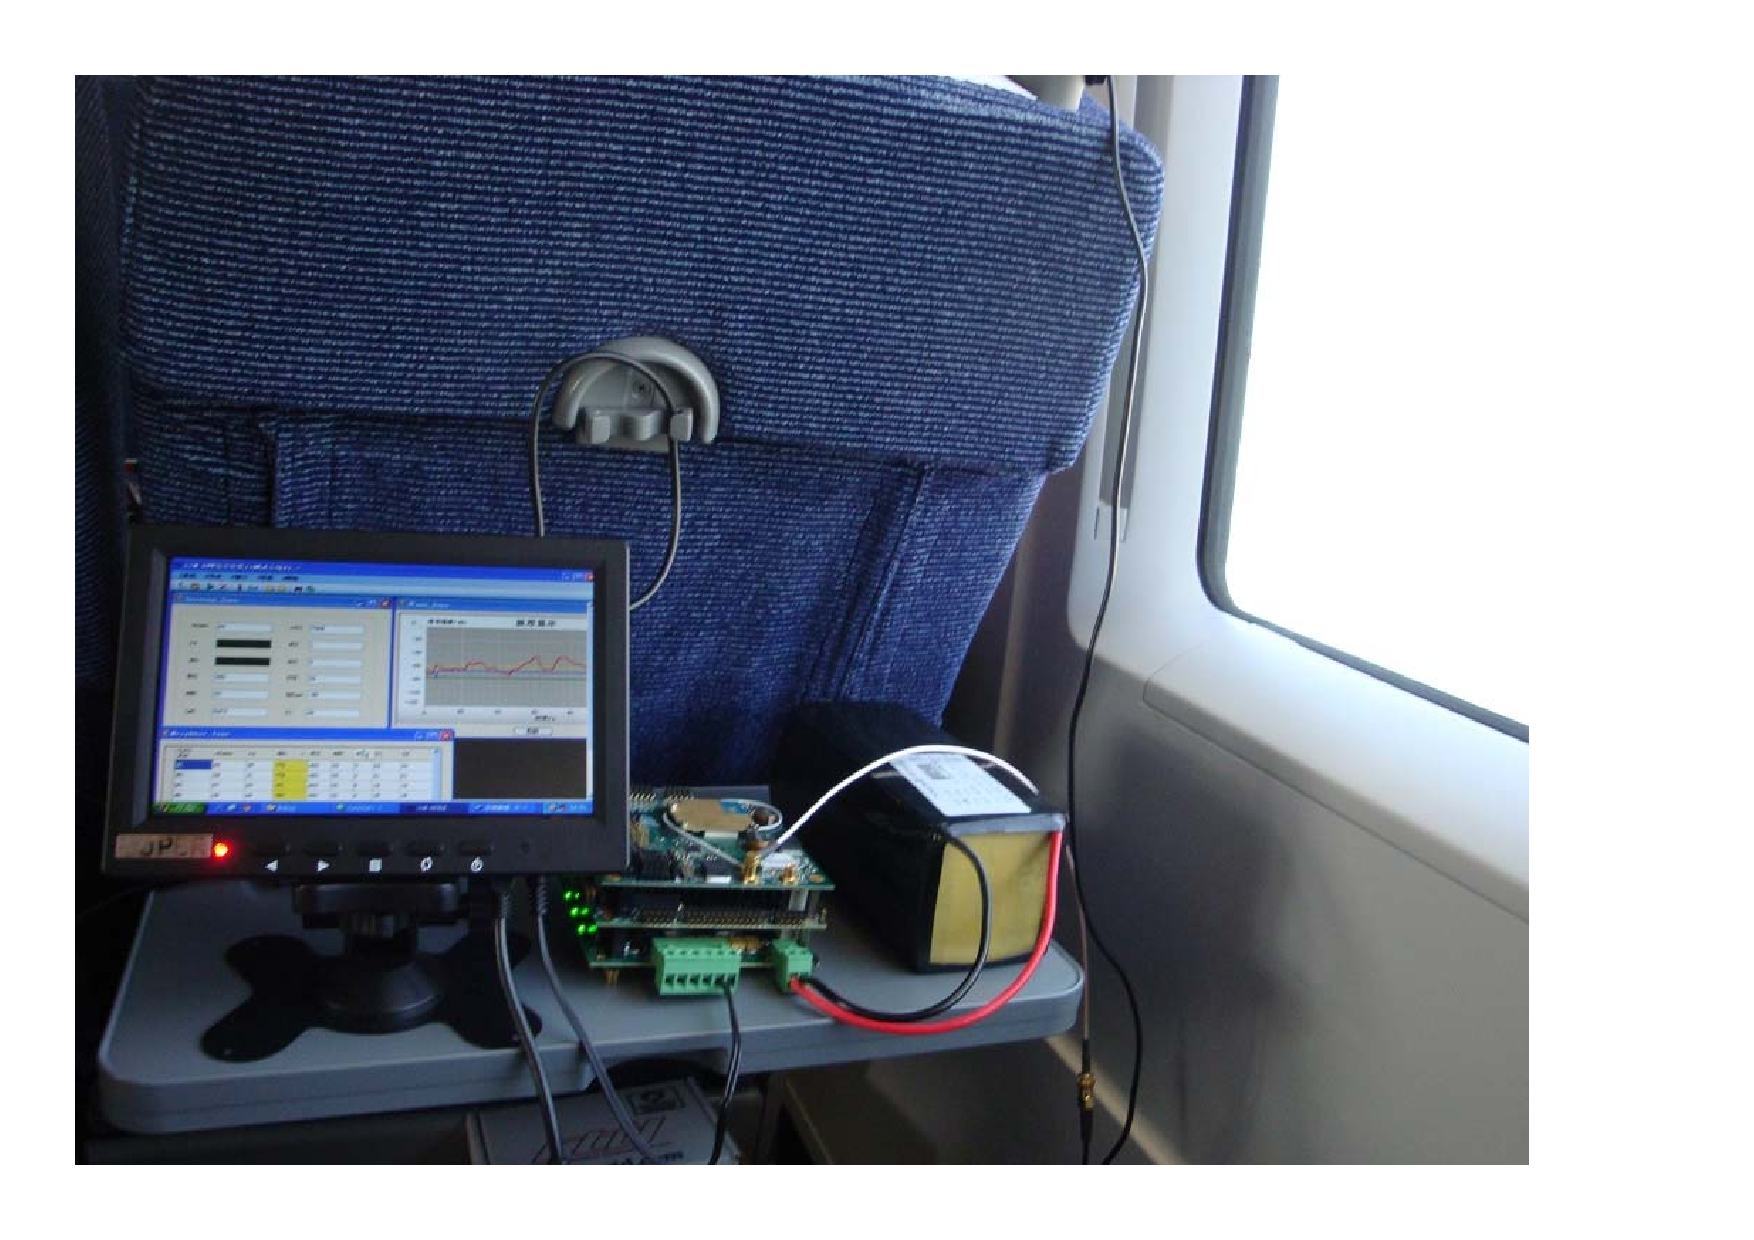
\includegraphics[width=2.5in]{chap5/platform.pdf}}
    \hspace{1cm}
\subfigure[Software Development]{
    \label{fig:software}
    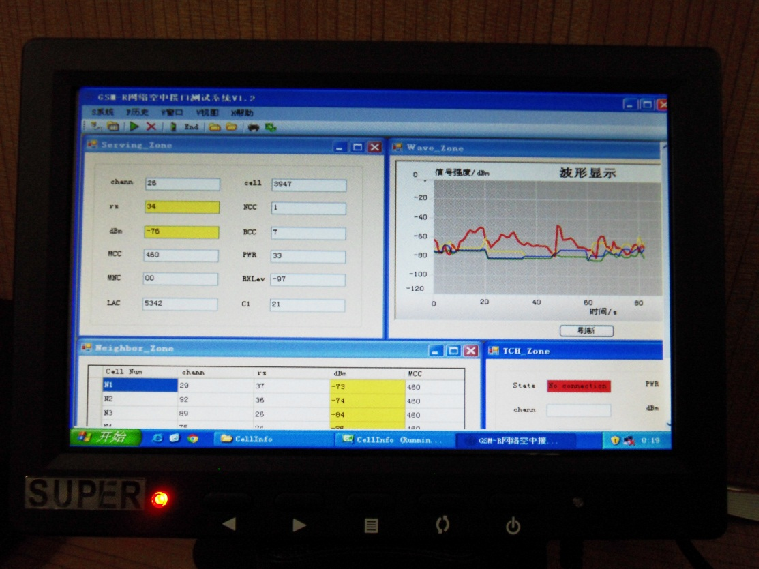
\includegraphics[width=2.5in]{chap5/softwareinterface.pdf}}
\bicaption[fig:platform]{GSM-R网络空中接口测试系统}{GSM-R网络空中接口测试系统}{Fig}{Um Interface Monitoring System for GSM-R Networks}
\end{figure}

As is illustrated in Fig.~\ref{fig:umframework}, the on-line estimation algorithm provides basic information to up-layer applications. The raw data of received signal strength is collected by GSM-R device, which is composed of the information of current cell and 6 neighbour cells. Then these data is processed by the on-line estimation algorithm to provide current network status and conduct next signal sampling. The system also provides received signal strength prediction based on the weighted averaging of signal samples, and gives warning information when the communication performance is lower than certain threshold. Since the system records the received signal strength of current and neighbour cells, the data can be used to make handover analysis and network optimization. Except the physical layer information, the system can also give quality of service of the link layer, including data traffic and voice service.

\section{802.11n网络链路质量测试}
\label{sec:80211n} 

This section describes the experimental platform and measurement setup for our channel measurement and prediction study in mobile 802.11n networks. We present a rate adaption algorithm, GradedR, to demonstrate the upper layer application of online PDR-RSS modeling framework.

\begin{figure}[!htp]
\centering

\includegraphics[width=5in]{chap5/testbed.pdf}
\bicaption[fig:testbed]{802.11n网络测试系统}{802.11n网络测试系统}{Fig}{Experiment testbed and measurement setup}
\end{figure}

We conduct both stationary and mobile experiments on two indoor platforms with different squares, as shown in Fig.~\ref{fig:testbed}. Each scenario covers both Line Of Sight (LOS) and None LOS (NLOS) radio transmissions, and stationary measurement is implemented (\textbf{P1} to \textbf{P11} in Fig.~\ref{testbed}) to obtain the multi-path fading and location difference features. Section \ref{modeling} mainly focus on stationary measurements to get the basic characteristics of PDR-RSS model and 802.11n PHY/MAC settings, and the online and mobile experiments (\textbf{r1} to \textbf{r6} in Fig.~\ref{fig:testbed}) will be discussed in Section \ref{experiment}.

The AP module used in our experiments is TP-LINK's TL-WRD4310 2.4/5GHz dual band gigabit router, which uses Atheros AR9580 radio chipset. It supports up to 3x3 MIMO and 300Mbps/450Mbps date rates for channel type of HT20/HT40. We conduct experiments with laptops in mobile, and the clients are using Atheros's 802.11n wireless card AR9380 with 2.4/5GHz dual band and 3 spatial streams. All the clients are running Linux kernel of 3.2.0-26 with modified ath9k wireless driver.

We conduct our experiments under 5.745GHz frequency band on channel 149, which encounters with less legacy interference. In both static and mobile experiments, UDP packets of 1500 bytes size are transmitted through \texttt{iperf}. To get accurate PDR measurement, some MAC layer mechanisms such as RTS/CTS and ACK are disabled, and also the spatial multiplexing power save mode. The packet delivery measurement of mobile 802.11n networks is carried out along different routes, as is illustrated in Fig.~\ref{fig:testbed}. The above experiments cover most of the key features of packet delivery in mobile 802.11n networks.


\begin{figure}[!htp]
\centering
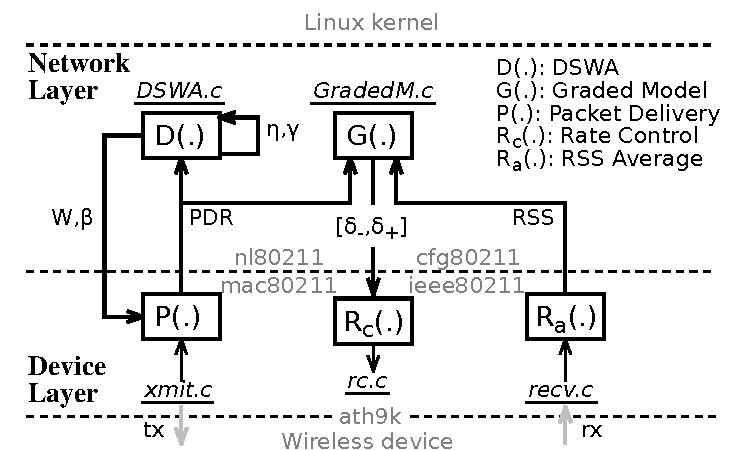
\includegraphics[width=5in]{chap5/framework.pdf}
\bicaption[fig:framework]{链路质量测试算法}{链路质量测试算法}{Fig}{Measurement framework and implementation on Linux systems}
\end{figure}

GradedR adopts DSWA to get accurate PDR measurement with low overhead, then chooses the suitable configuration according to HT/GI/MCS index. The pseudo code of above process is shown in Procedure \ref{fig:alg_pdr}, and the PDR threshold in GradedM.c is set to \{$P_{thrl},P_{thrh}$\}=\{$10\%,90\%$\}. When the selected MCS is far away the right bound of its transition window, GradedR will choose a new configuration to acquire a higher data rate. On the contrast, it will reduce the data rate when current PDR falls into the transition window. Given the characterization results in Section \ref{modeling}, we only select SGI as the final rate adaptation step when the link quality is still poor running at the highest rates of LGI.

\begin{algorithm}[!htp]
\floatname{algorithm}{Procedure}
\renewcommand{\algorithmicrequire}{\textbf{Input:}}
\renewcommand{\algorithmicensure}{\textbf{Output:}}
\caption{GradedM $\rightarrow$ DSWA $\rightarrow$ GradedR}
\label{alg_pdr}
\begin{algorithmic}[1]
\Require tx-complete (packets transmitted event)
\Ensure  rate-index (rate selection indexes of HT/GI/MCS)
\State{// DSWA(pdr-last,pdr-now): return averaging window length $W$ and sliding factor $\beta$, update $\gamma$ and $\eta$}
\State{// GradedM(pdr,rss): update the graded-table and sort it into MCS selection sequences, return ht-gi-mcs-index}
\State{// GradedR(ht-gi-mcs-index): return ht-gi-mcs, ensure current PDR out of the transition window with the highest available data rate}
\If{pdr-now $<P_{thrh} |$ rss-now $<\delta_+$}
\State{graded-talbe $\gets$ GradedM(pdr-now,rss-now);} // rc.c
\State{rate-index $\gets$ down-rate-mcs(ht-gi-mcs-table);}
\EndIf
\If{graded-sens - rss-now $>$ high-limit-to-gray}
\State{rate-index $\gets$ up-rate-mcs(ht-gi-mcs-table);}
\EndIf
\State \Return{\{tx-status,rate-index\};}
\end{algorithmic}
\end{algorithm}

We implemented above algorithm on Linux systems with modified \texttt{ath9k} wireless driver. Fig.~\ref{fig:framework} illustrates the software architecture, which is composed of both network layer and device layer components. The network layer conducts DSWA calculations to determine averaging intervals and sliding factor, and makes GradedT update to get rate selection indexes. On the device layer, it is driven by transmitting and receiving events that execute PDR computation and RSS averaging respectively. The rate indexes are also selected on device layer according to results of network layer when the PDR or RSS is lower than transmission threshold.
